\documentclass{homework}
\usepackage[utf8]{inputenc}
\usepackage{amsmath}
\usepackage{amssymb}
\usepackage{braket}
\usepackage{graphicx}

% CHANGE THE FOLLOW THREE LINES!
\newcommand{\hwname}{Vaansh Lakhwara}
\newcommand{\hwemail}{ID: 401147641}
\newcommand{\hwnum}{2}

% CHANGE THESE ONLY ONCE PER CLASS
\newcommand{\hwtype}{Assignment}
\newcommand{\hwclass}{COMP 335}

\begin{document}
\maketitle

\question

\textbf{(a)}\\
\begin{center}
    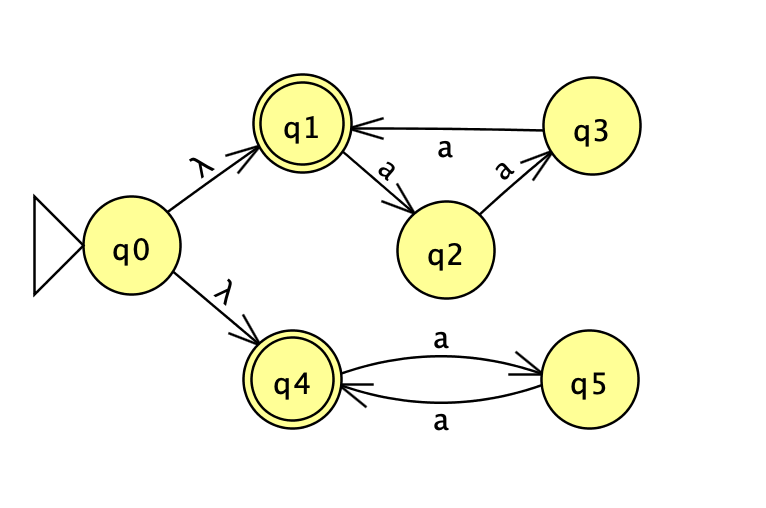
\includegraphics{A2Q1.png}\\
\end{center}

\textbf{(b)}\\
Let L represent language represented by M\\
$\therefore$, L = \{(a)$^i$, where i is divisible by 2 or 3, and i $\geq$\ 0\}\\

\question
\textbf{(a)}\\
A simple description of L without referencing parameter k would be defining L as:\\
L=\{1x : x$\in$\{0,1\}$^*$, x has at least one 1\}\\
\newline
\underline {Proof:}\\
Taking into consideration what is given in the description, the minimum value of k is 1\\
$\therefore$, at k=1, L=\{1x : x$\in$\{0,1\}$^*$\}\\
\newline
\newline
However, since y is \{0,1\}*, and has at least k 1’s, y must also have at least one 1, which is why finally L can be represented as:\\
\newline
L=\{1x:x$\in$\{0,1\}$^*$, x has at least one 1\}\\

\textbf{(b)}\\
\begin{center}
    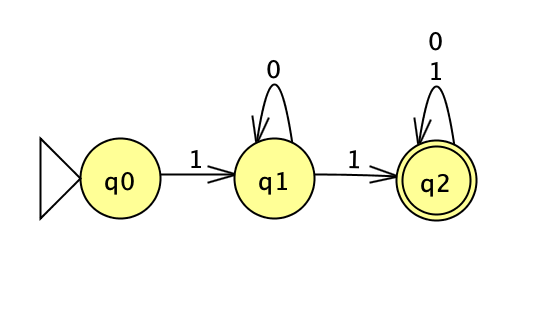
\includegraphics{A2Q2.png}\\
\end{center}

\textbf{(c)}\\
No, L cannot be accepted by an NFA with fewer than three states. As defined and proved in (a), there has to be at least two 1's. However, there is no possible configuration  using fewer than three states.\\

\question
\textbf{(a)}\\
\begin{center}
    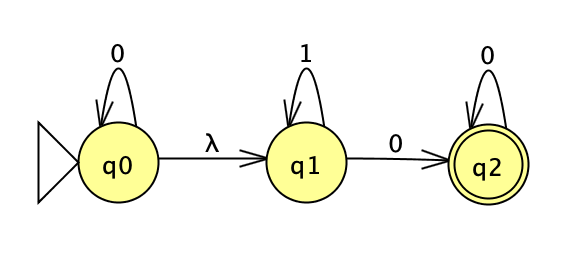
\includegraphics{A2Q3A.png}
\end{center}
This diagram accepts any number of 0's followed by any number of 1's, which precedes at least one 0, as specified in the language\\
\textbf{(b)}\\
\begin{center}
    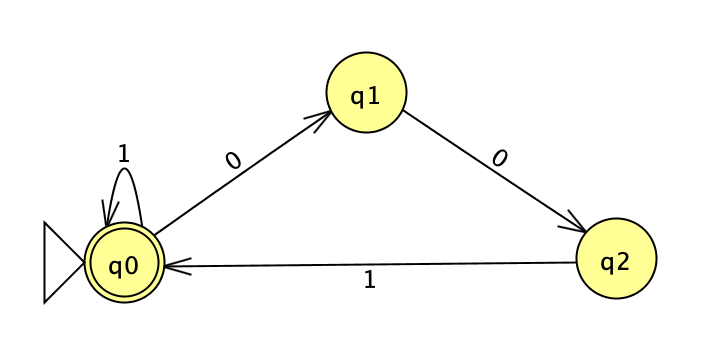
\includegraphics{A2Q3B.png}
\end{center}
This diagram accepts any number of 1's followed by two 0's and 1's that can be repeated any number of times, which precedes at least one 0, as specified in the language\\
\end{document}